\subsection{APIs}


\subsubsection{Web Storage}

El almacenamiento web de HTML5 permite guardar información y datos en la computadora del usuario que acceda a nuestro sitio y genera datos, con esto, podemos acceder a ellos si es que el usuario entra en otro momento, evitamos enviar la información nuevamente (si es que ya fue almacenada), tomarla si ya fue almacenada, es más seguro, etc. Para utilizar esta API, es necesario conocer JavaScript.

\textbf{Tipos del almacenamiento web.}

\begin{itemize}
    \item \textbf{sessionStorage()}: crea una sesión y almacena información en la misma; esta información y sesión serán destruidas una vez el usuario cierre el buscador.
    \item \textbf{localStorage()}: crea una sesión sin expiración y almacena la información en la máquina del usuario.
\end{itemize}

\textbf{Operaciones con el almacenamiento web.}

Todas estas operaciones son trabajadas con JavaScript, ya sea con un almacenamiento local o de sesión, los datos son almacenados por medio de un \textbf{par llave/valor}:
\begin{lstlisting}
    // Guardando datos.
    localStorage.setItem("llave1", "valor1");
    sessionStorage.setItem("llave1", "valor1");

    // Obteniendo e imprimendo datos guardados.
    alert(localStorage.getItem("llave1"));
    alert(sessionStorage.getItem("llave1"));

    // Eliminando un dato.
    localStorage.removeItem("llave1");
    sessionStorage.removeItem("llave1");

    // Eliminando todos los datos.
    localStorage.clear();
    sessionStorage.clear();
\end{lstlisting}


\subsubsection{Geolocation}

Es la ubicación actual del usuario (siendo más precisa en dispositivos con GPS), este dato compromete la privacidad de los individuos, por lo que el sitio web debe preguntar al usuario si este desea compartir su ubicación:
\begin{center}
    \textit{navigator.geolocation.getCurrentPosition();}
\end{center}

Donde los parámetros de \textit{getCurrentPosition()} son:
\begin{itemize}
    \item \textbf{showLocation}: obligatorio, establece un método que recibe la información de la ubicación.
    \item \textbf{ErrorHandler}: opcional, establece un método en caso de que un error ocurra en la llamada asíncrona.
    \item \textbf{Options}: opcional, define algunas opciones a la hora de recibir la información de la ubicación.
\end{itemize}

\textbf{Presentando la información}

La información de la ubicación puede ser presentada en las siguientes formas:
\begin{itemize}
    \item \textbf{Geodetic}: es presentada según latitud y longitud.
    \item \textbf{Civic}: es presentada de una manera más simple para una persona, por medio de ciudades y otros datos civiles.
\end{itemize}

La \textit{Figura \ref{fig: 18}} lo explica mejor:
\begin{figure}[H]
    \centering
    \caption{Formas de presentar la geolocalización}
    \label{fig: 18}
    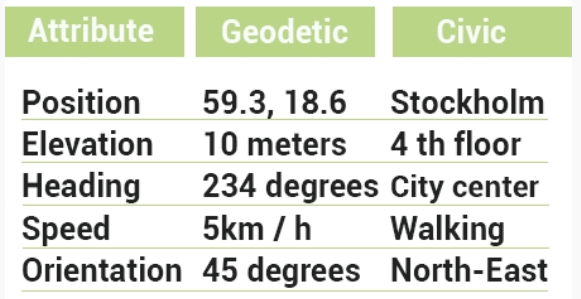
\includegraphics[width=7cm]{ss_html/geolocation.png}
\end{figure}

\textit{Nota}: el método \textbf{getCurrentPosition()} siempre regresa un objeto, donde los atributos \textit{latitude}, \textit{longitude} y \textit{accuracy} siempre son retornados.

El siguiente ejemplo nos ayudará a comprender la forma de trabajar la geolocalización (\textit{Figura \ref{fig: 19}}):
\begin{lstlisting}
    <p>Click the button to get your coordinates.</p>
    <!-- Botón que al presionarlo llama a la función "getLocation" del script insertado. -->
    <button onclick="getLocation()">Try It</button>
            
    <p id="demo"></p>

    <script>
        var x = document.getElementById("demo");

        // Obtiene la localización del buscador.
        function getLocation() {
            if (navigator.geolocation) {
                navigator.geolocation.getCurrentPosition(showPosition);
            }
            else { 
                x.innerHTML = "Geolocation is not supported by this browser.";
            }
        }
        // Muestra la localización en HTML.
        function showPosition(position) {
            x.innerHTML = "Latitude: " + position.coords.latitude + 
            "<br>Longitude: " + position.coords.longitude;
        }
    </script>
\end{lstlisting}
\begin{figure}[H]
    \centering
    \caption{Ejemplo de geolocalización}
    \label{fig: 19}
    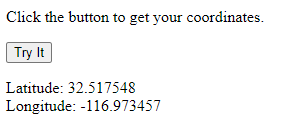
\includegraphics[width=7cm]{ss_html/geolocation_1.png}
\end{figure}


\subsubsection{Drag \& Drop}

Todos las etiquetas y objetos HTML pueden ser \textit{draggable}, solamente añada el atributo \textbf{draggable} con su valor \textbf{true}:
\begin{center}
    \textit{$<$img draggable="true" /$>$}
\end{center}

Esto es por parte de HTML, la API del Drag \& Drop está basada en un evento JavaScript, como vemos en el siguiente ejemplo:
\begin{lstlisting}
    <html>
        <head>
            <!-- Script interno. -->
            <script>
                // Permite el arrastrado de etiquetas.
                function allowDrop(ev) {
                    ev.preventDefault();
                }
                // Realiza la acción de arrastrar la etiqueta y su información.
                function drag(ev) {
                    ev.dataTransfer.setData("text", ev.target.id);
                }
                // Realiza la acción de soltar la etiqueta y su información.
                function drop(ev) {
                    ev.preventDefault();
                    var data = ev.dataTransfer.getData("text");
                    ev.target.appendChild(document.getElementById(data));
                }
            </script>
        </head>
        <body>
            <!-- Establece contenedor para soltar un elemento. -->
            <div id="box" ondrop="drop(event)" ondragover="allowDrop(event)"
                style="border:1px solid black; width:200px; height:200px">
            </div>
            <!-- Etiqueta capaz de ser arrastrada. -->
            <img id="image" src="sample.jpg" draggable="true"
                ondragstart="drag(event)" width="150" height="50" alt="" />
        </body>
    </html>
\end{lstlisting}

La explicación es la siguiente: cuando una etiqueta u objeto es arrastrado (dragged), el atributo \textbf{ondragstart} llama a una función: \textbf{drag(event)}, el cual especifica la información a arrastrar. El método \textbf{dataTransfer.setData()} especifica el tipo y valores de la información arrastrada; este método te permite acceder también a la información del objeto o etiqueta arrastrada, regresará cualquier información asignada al tipo dado en el método \textbf{setData()}, este tipo puede ser el ID del elemento arrastrado (imágenes, videos, audios, paneles, etc).

El evento \textbf{ondragover} especifica dónde la información puede ser soltada. Por defecto, la información o etiquetas no pueden ser soltadas sobre otras etiquetas, por lo que debemos prevenir esto mediante el método \textbf{preventDefault()}; permite prevenir al buscador que se cambiará la forma por defecto para manejar la información (\textit{por defecto está como enlace a soltar, no otros objetos}).

Al soltar el clic y soltar (drop) la etiqueta, objeto o información, ocurre el evento \textit{drop}. El atributo \textbf{ondrop} va ligado al objeto que recibirá lo que sea que se le suelte, a quien recibirá la información u objeto.


\subsection{SVG}

SVG significa \textbf{Scalable Vector Graphics} (Gráficos vectoriales escalables), y es utilizado para dibujar figuras con un estilo HTML. En HTML funciona tanto como una etiqueta, como en un formato de imagen para una etiqueta \textit{img}, y la podemos utilizar para dibujar cajas, líneas, círculos, textos y gráficas en imágenes (recordemos que los formatos \textit{.svg} puede ser aumentada o disminuida de tamaño sin perder calidad).
\begin{center}
    \textit{$<$img src="imagen.svg" alt="" height="300" /$>$}
\end{center}

La etiqueta \textbf{svg} debe tener los atributos \textit{width} y \textit{height} de manera obligatoria, para dimensionar el panel o espacio donde será dibujada la figura; tome en cuenta que, si este espacio de dibujo es menor al tamaño de la figura, esta se dibujará incompleta en el espacio de dibujo.


\subsubsection{Dibujando figuras}

Crearemos un \textbf{círculo} en el siguiente ejemplo con su visualización (\textit{Figura \ref{fig: 20}}):
\begin{lstlisting}
    <!-- Crea un panel de dibujo SVG de 3000x3000 píxeles. -->
    <svg width="3000" height="3000">
        <!-- Dibuja un círculo de radio 50, de color rojo y borde negro.. -->
        <circle cx="100" cy="150" r="50" fill="red" stroke="black"/>
    </svg>
\end{lstlisting}
\begin{figure}[H]
    \centering
    \caption{Dibujando un círculo con SVG}
    \label{fig: 20}
    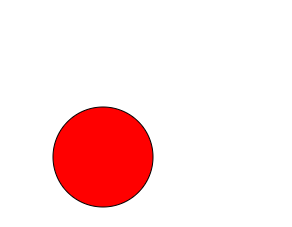
\includegraphics[width=7cm]{ss_html/svg_circle.png}
\end{figure}

Donde:
\begin{itemize}
    \item \textbf{cx}: coordenada \textit{x}, empuja el centro del círculo desde la izquierda de la página.
    \item \textbf{cy}: coordenada \textit{y}, empuja el centro del círculo desde la parte superior de la página.
    \item \textbf{r}: radio del círculo.
    \item \textbf{fill}: rellena la figura con un color.
    \item \textbf{stroke}: añade un borde de color a la figura (atributo más personalizable en CSS).
\end{itemize}

Como podemos suponer, hay ciertos atributos únicos para cada figura posible para dibujar, otros son más generales, como \textit{fill} o \textit{stroke}.

Ahora crearemos un \textbf{rectángulo} en el siguiente ejemplo con su visualización (\textit{Figura \ref{fig: 21}}):
\begin{lstlisting}
    <svg width="3000" height="3000">
        <!-- Dibuja un rectángulo de 300x100 píxeles, de color rojo y borde negro. -->
        <rect width="300" height="100" x="30" y="30" fill="red" stroke="black" />
    </svg>
\end{lstlisting}
\begin{figure}[H]
    \centering
    \caption{Dibujando un rectángulo con SVG}
    \label{fig: 21}
    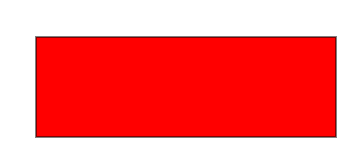
\includegraphics[width=7cm]{ss_html/svg_rect.png}
\end{figure}

Donde:
\begin{itemize}
    \item \textbf{width}: ancho del rectángulo.
    \item \textbf{height}: altura del rectángulo.
    \item \textbf{x}: coordenada \textit{x}, igual que el atributo \textit{cx}.
    \item \textbf{y}: coordenada \textit{y}, igual que el atributo \textit{cy}.
\end{itemize}

Una \textbf{línea} puede ser dibujada siguiendo el ejemplo a continuación, el resultado puede apreciarse en la \textit{Figura \ref{fig: 22}}:
\begin{lstlisting}
    <svg width="3000" height="3000">
        <!-- Dibuja una línea negra con inicio en x(10,10) y y(200,100). -->
        <line x1="10" y1="10" x2="200" y2="100" stroke="black" />
    </svg>
\end{lstlisting}
\begin{figure}[H]
    \centering
    \caption{Dibujando una línea con SVG}
    \label{fig: 22}
    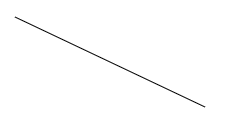
\includegraphics[width=7cm]{ss_html/svg_line.png}
\end{figure}

Donde:
\begin{itemize}
    \item \textbf{x1}: coordenada \textit{x} para el punto inicial de la línea, empuja este punto desde la izquierda de la página.
    \item \textbf{y1}: coordenada \textit{y} para el punto inicial de la línea, empuja este punto desde la parte superior de la página.
    \item \textbf{x2}: coordenada \textit{x} para el punto terminal de la línea, empuja este punto desde la izquierda de la página.
    \item \textbf{y2}: coordenada \textit{y} para el punto terminal de la línea, empuja este punto desde la parte superior de la página.
\end{itemize}

Una \textbf{polilínea} (una línea tras otra) puede ser dibujada siguiendo el ejemplo a continuación, el resultado puede apreciarse en la \textit{Figura \ref{fig: 23}}:
\begin{lstlisting}
    <svg width="3000" height="3000">
        <!-- Dibuja un camino de líneas que forman dos triángulos uno al lado del -->
        <!-- otro con relleno negro. -->
        <polyline points="100 100, 150 150, 200 100, 250 150, 300 100" stroke="black" />
    </svg>
\end{lstlisting}
\begin{figure}[H]
    \centering
    \caption{Dibujando una ruta con SVG}
    \label{fig: 23}
    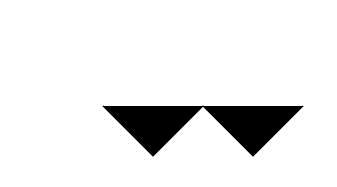
\includegraphics[width=7cm]{ss_html/svg_polyline.png}
\end{figure}

Donde:
\begin{itemize}
    \item \textbf{points}: son las coordenadas \textit{x}, \textit{y} de los puntos que seguirá la ruta, se separan únicamente por comas.
    \item \textbf{stroke}: en este caso, el atributo colorea por completo la ruta.
\end{itemize}

Una \textbf{elipse} puede ser dibujada siguiendo el ejemplo a continuación, el resultado puede apreciarse en la \textit{Figura \ref{fig: 24}}:
\begin{lstlisting}
    <svg width="3000" height="3000">
        <!-- Dibuja una elipse roja con borde negro. -->
        <ellipse cx="200" cy="100" rx="150" ry="70" fill="red" stroke="black" />
    </svg>
\end{lstlisting}
\begin{figure}[H]
    \centering
    \caption{Dibujando una elipse con SVG}
    \label{fig: 24}
    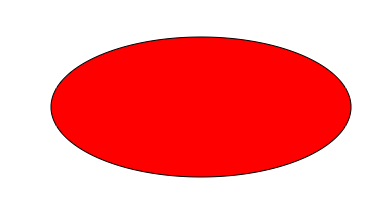
\includegraphics[width=7cm]{ss_html/svg_ellipse.png}
\end{figure}

Donde:
\begin{itemize}
    \item \textbf{cx}: coordenada \textit{x}, aplicable igual al círculo.
    \item \textbf{cy}: coordenada \textit{y}, aplicable igual al círculo.
    \item \textbf{rx}: tamaño del radio horizontal de la elipse.
    \item \textbf{ry}: tamaño del radio vertical de la elipse.
\end{itemize}

Un \textbf{polígono} puede ser dibujada siguiendo el ejemplo a continuación, el resultado puede apreciarse en la \textit{Figura \ref{fig: 25}}:
\begin{lstlisting}
    <svg width="3000" height="3000">
        <!-- Dibuja un polígono rojo con borde negro. -->
        <polygon points="100 100, 200 200, 300 0" fill="red" stroke="black" />
    </svg>
\end{lstlisting}
\begin{figure}[H]
    \centering
    \caption{Dibujando un polígono con SVG}
    \label{fig: 25}
    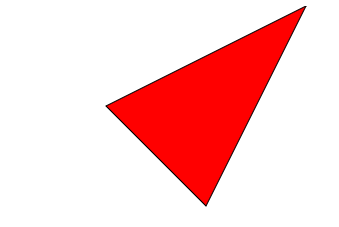
\includegraphics[width=7cm]{ss_html/svg_polygon.png}
\end{figure}

Donde:
\begin{itemize}
    \item \textbf{points}: son las coordenadas \textit{x}, \textit{y} de los puntos que seguirá la ruta, se separan únicamente por comas.
\end{itemize}

\textit{Nota}: recuerde que el atributo \textit{stroke} puede ser modificado y personalizado a profundidad con CSS, al igual que el atributo \textit{fill}.


\subsubsection{Animaciones y rutas}

Además de crear figuras, svg puede crear animaciones con la etiqueta \textbf{animate} y sus siguientes atributos:
\begin{itemize}
    \item \textbf{attributeName}: especifica el atributo o variable que será afectada por la animación. Los valores que se le pueden dar a este atributo pueden ser: x, y, rx, ry, cx, cy, r, etc.
    \item \textbf{from}: valor inicial del atributo de la animación.
    \item \textbf{to}: valor final del atributo de la animación.
    \item \textbf{dur}: duración de la animación (3s, 4s, 10s).
    \item \textbf{fill}: indica qué ocurre con el valor del atributo o variable cuando la animación termina. Puede adoptar el valor "freeze" (mantiene el valor final que tuvo el atributo) o "remove" (resetea el valor del atributo).
    \item \textbf{repeatCount}: número de veces que se repetirá la animación. Puede utilizar el valor "indefinite" para que la animación se repita indefinidamente.
\end{itemize}

Pondremos un ejemplo donde un cuadrado baja infinitamente a continuación y puede ejecutarlo en su buscador:
\begin{lstlisting}
    <svg width="1000" height="1000">
        <rect width="150" height="150" fill="orange" stroke="black">
            <animate attributeName="y" from="0" to="300" dur="3s" fill="freeze" repeatCount="indefinite"/> 
        </rect>
    </svg>
\end{lstlisting}

Una \textbf{ruta} puede ser definida con la etiqueta \textbf{path}, su atributo \textbf{d} es la que establece cómo será la ruta; al igual que el dibujado de figuras en la sección anterior, se utilizan coordenadas \textit{x}, \textit{y}, sin embargo, el atributo \textbf{d} puede contener valores adicionales a las coordenadas:
\begin{itemize}
    \item \textbf{M}: move to (punto inicial de la ruta).
    \item \textbf{L}: line to (línea diagonal, horizontal o vertical).
    \item \textbf{H}: horizontal line to.
    \item \textbf{V}: vertical line to
    \item \textbf{C}: curve to.
    \item \textbf{S}: smooth curve to.
    \item \textbf{Q}: quadratic Bézier curve.
    \item \textbf{T}: smooth quadratic Bézier curve to.
    \item \textbf{A}: elliptical Arc.
    \item \textbf{Z}: close path (cierra la ruta).
\end{itemize}

Como puede ver, estos valores adicionales están en mayúsculas, esto indica que la ruta tendrá una \textbf{posición absoluta}, si utiliza letras minúsculas la \textbf{posición será relativa}.

Creamos una ruta triangular a continuación, puede ver el resultado en la \textit{Figura \ref{fig: 26}}:
\begin{lstlisting}
    <svg width="3000" height="3000">
        <!-- Dibuja una ruta color negro. -->
   	<path d="M 0 0 L200 200 L400 0 Z" stroke="black" fill="none" />
    </svg>
\end{lstlisting}
\begin{figure}[H]
    \centering
    \caption{Dibujando una ruta con SVG y path}
    \label{fig: 26}
    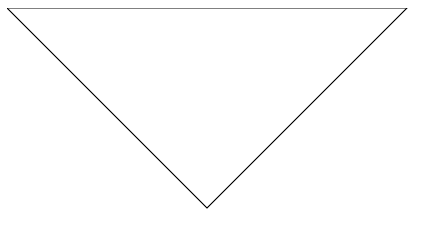
\includegraphics[width=7cm]{ss_html/svg_path.png}
\end{figure}

Nuestra área de dibujo debe tener un punto de inicio para dibujar la ruta, \textit{M 0 0} crea este punto de inicio, \textit{L200 200} crea una línea entre las coordenadas (0, 0) y (200, 200), \textit{L400 0} crea una línea entre las coordenadas (200, 200) y (400, 0), finalmente, \textit{Z} dibuja una línea entre el último punto creado (400, 0) y el punto inicial (0, 0); de esta manera, podemos conseguir crear rutas en nuestros documentos HTML. Nótese que el atributo \textit{fill} tiene el valor \textbf{none}, esto evita que la ruta se coloree completamente (cosa que ocurrió dibujando polilíneas).
